\documentclass[12pt,a4paper]{report}

\usepackage[utf8]{inputenc}
\usepackage{natbib}
\usepackage{graphicx}

% Margins
\usepackage{geometry}
\geometry{a4paper,top=2cm,bottom=2cm,left=2cm,right=2cm,heightrounded,bindingoffset=5mm}

\begin{document}

\begin{titlepage}
	\centering
	
	% Title
	\rule[0.5ex]{\linewidth}{2pt}\vspace*{-\baselineskip}\vspace*{3.2pt}
	\rule[0.5ex]{\linewidth}{1pt}\\[\baselineskip]
	
	{\huge\bfseries Smart thermostat}\\[4mm]
	{\large Internet of Things Project}\\[3mm]
	
	\rule[0.5ex]{\linewidth}{1pt}\vspace*{-\baselineskip}\vspace{3.2pt}
    \rule[0.5ex]{\linewidth}{2pt}\\[\baselineskip]
    
	% Polimi logo
	\vspace{2cm}
	
\includegraphics[width=0.4\textwidth]{images/Polimi.png}\par
	\vspace{2mm}
	{\large Master's Degree in Computer Science and Engineering\\
	\vspace{2mm}
	\textsc{Politecnico di Milano}}

    % Author
    \vspace{3cm}
	{\Large Michele Scuttari\\
	920679\\
	michele.scuttari@mail.polimi.it\par}

	
    % Bottom of the page
    \vfill
	{\large July 2019 \par}
	\vspace{1cm}
\end{titlepage}

\section*{Introduction}
The project consists in the development of a smart thermostat, composed by a set of sensors and a client that collects and shows the data produced by them. Each sensor is also linked to its room systems (cooling, heating and ventilation), which can be enabled through the client dashboard.

\section*{Sensors}
The sensors have been developed using the \textit{Contiki 2.7} operating system and simulated using \textit{Cooja}.\\[8 pt]
Their development has been thought in a modular way with respect to the capabilities it should offer: at compile time, the non required systems can be disabled by just setting their macro to zero. This way, a thermostat that for example has only the cooling and ventilation systems available, can have the heating part disabled without a radical change of its code.\\[8 pt]
Furthermore, the systems activation / deactivation is done through their dedicated functions, which are called by the core logic of the thermostat. Thanks to this design choice, the core logic is fully decoupled from the environment specific implementation and real thermostats just have to specify the way the systems can be turned on and off (which can happen for example by setting some pins high or by sending a network request). Being this just a prototype, these functions just turn on or off the respective LED (blue for cooling, red for heating and green for ventilation).\\[8 pt]
The same decoupling strategy has been adopted for the temperature probing. Being this not a real environment, an internal simulation has been implemented by means of an independent process, in order to simulate the temperature change. As for the systems, also the simulation can be disabled quickly by just setting its macro to zero.\\[8 pt]
Finally, each sensor implements a CoAP server which exposes the following resources to the network:
\begin{itemize}
    \item \textbf{/temperature} [GET]: reports the last temperature reading; can be observed.
    \item \textbf{/systems} [GET]: reports whether each system is active or not.
    \item \textbf{/systems/cooling} [POST]: start or stop the cooling system.
    \item \textbf{/systems/heating} [POST]: start or stop the heating system.
    \item \textbf{/systems/ventilation} [POST]: start or stop the ventilation system.
\end{itemize}

\section*{Border router}
The sensors runs on a RPL network and requires a border router to communicate with the external IP network. For this project the default border router implementation, distributed together with Contiki, has been used.\\[8 pt]
The default SLIP tool (\textit{tunslip6}) has been used to assign the prefix to the network.\\[8pt]
The web server of the border router has also been kept enabled, in order to quickly see the addresses of the sensors, and can be reached at the address \textit{coap://[aaaa::212:7401:1:101]}.

\section*{Client}
The client has been developed using \textit{Node-RED} together with its \textit{CoAP} plugin (\textit{node-red-contrib-coap}).\\[8pt]
It consists in a single flow conceptually divided in three parts.
\begin{enumerate}
    \item \textbf{Sensors control and data collection}\\
    Allows the user to activate the systems of each thermostat and retrieve the current temperature by observing its temperature resource. The received temperature is stored in a "one minute living" array to allow the operations executed by the second part.
    \item \textbf{Data elaboration and ThingSpeak publication}\\
    Every minute, the acquired temperature readings are elaborated in order to compute the average for each sensor and the home one. The results are then published using MQTT to two different ThingSpeak channels and the aformentioned arrays are emptied to allow data collection for the following minute.\\
    Furthermore, if the last sensor temperature is out of the desired range, the system sends an email alert to the user. This temperature check is placed in this part and not the first one in order to avoid to send an email every 5 seconds (frequency of temperature sensing) in case of problems.
    \item \textbf{ThingSpeak subscription}\\
    Subscribes to the previous channels in order to display the last hour temperatures.
\end{enumerate}
The thermostats configurations and the temperature readings are stored in flow level variables. This way, also the other nodes can easily access to them.\\[8 pt]
As regards the user interface, Node-RED doesn't allow a dynamic instantiation of the dashboard items and therefore there are sequences of repeated blocks according to the number of thermostats. The difference between one repeated sequence and another is just the thermostat the blocks are referring to and the correspondent section in the dashboard.

\section*{Screenshots}
What follow are some screenshot taken while the whole system is operating.\\[8 pt]
\subsection*{Simulation network}
\begin{minipage}{0.35\linewidth}
    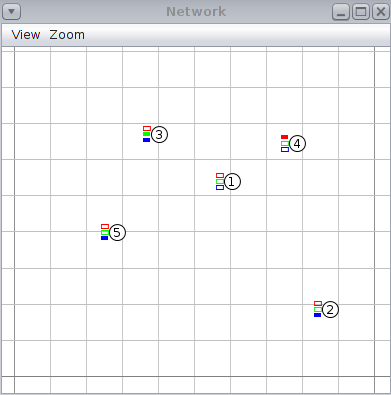
\includegraphics[width=\linewidth]{images/cooja-network.png}
\end{minipage}\hfil
\begin{minipage}{0.55\linewidth}
\begin{tabular}{cccc}
\textbf{Node} & \textbf{Type} & \textbf{Active systems}\\
1 & Border router & -\\
2 & Thermostat & Cooling\\
3 & Thermostat & Cooling, ventilation\\
4 & Thermostat & Heating\\
5 & Thermostat & Cooling\\
\end{tabular}
\end{minipage}

\subsection*{Client dashboard}
\begin{center}
    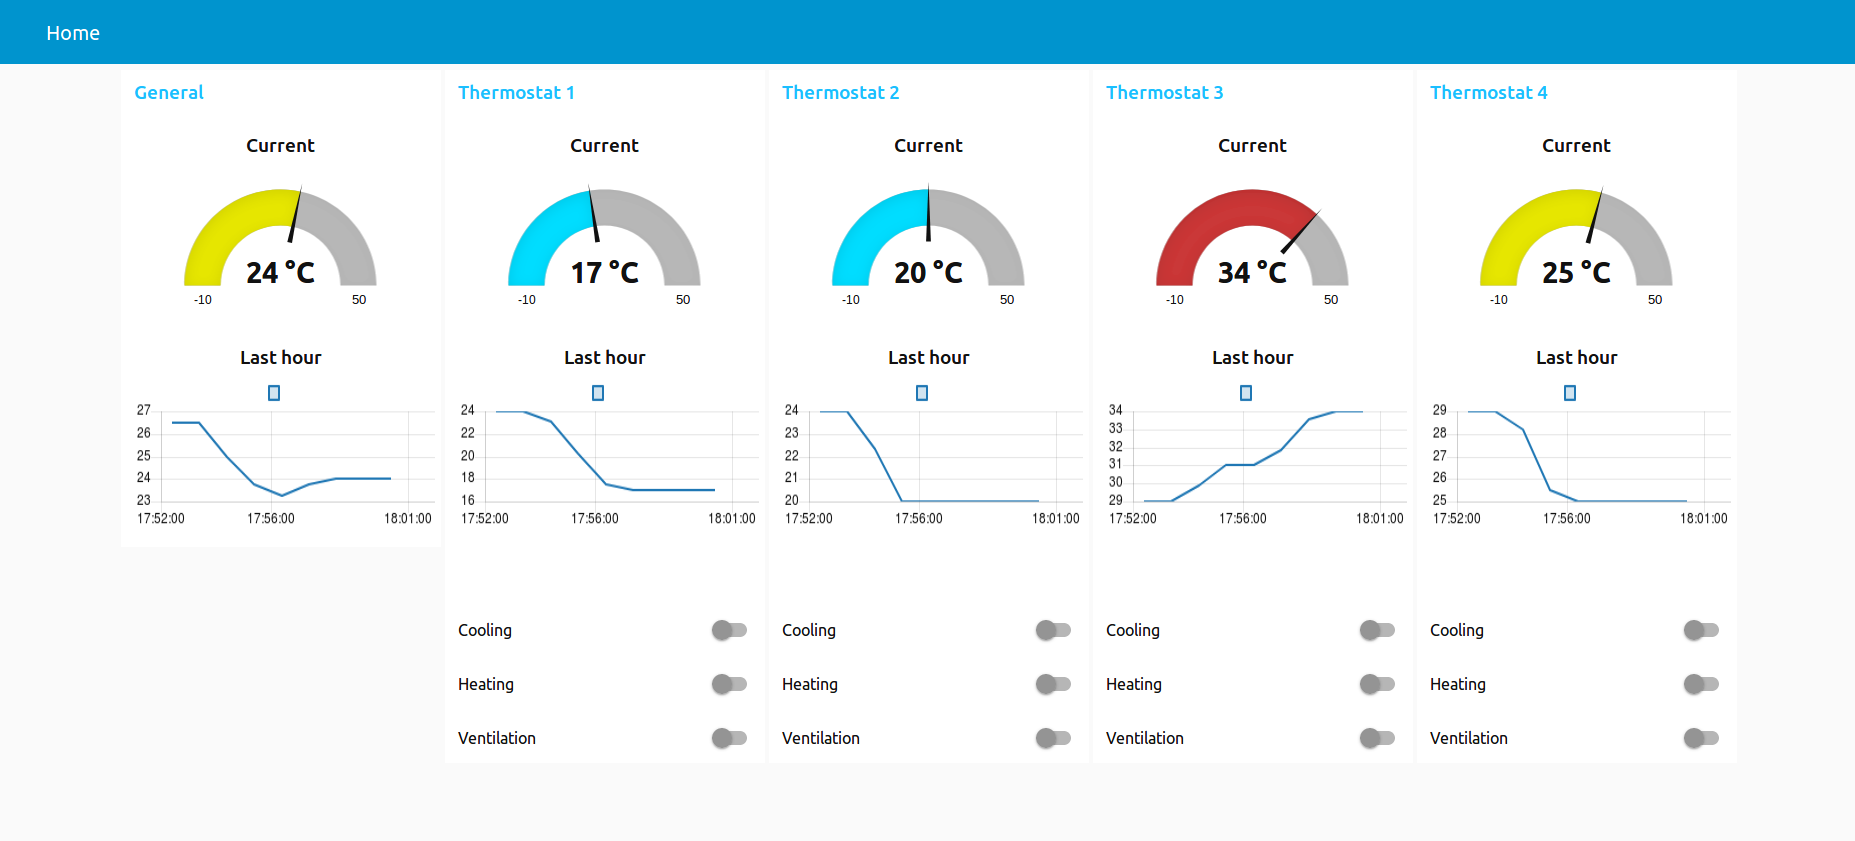
\includegraphics[width=\linewidth]{images/dashboard.png}
\end{center}

\subsection*{ThingSpeak - Home average temperature channels}
\begin{center}
    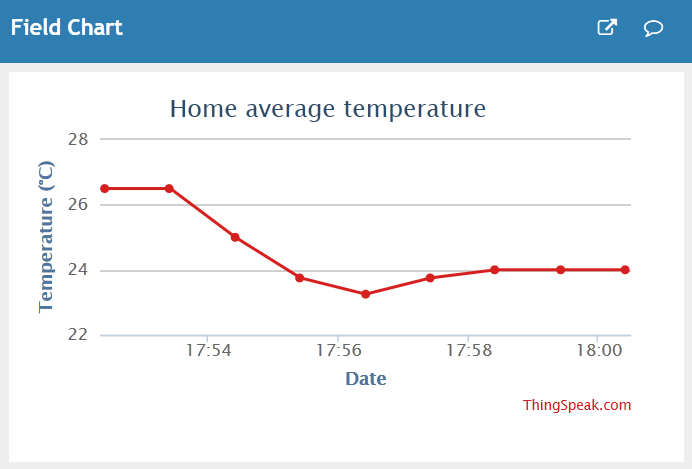
\includegraphics[width=0.5\linewidth]{images/thingspeak-home.png}
\end{center}

\subsection*{ThingSpeak - Thermostats average temperatures}
\begin{center}
    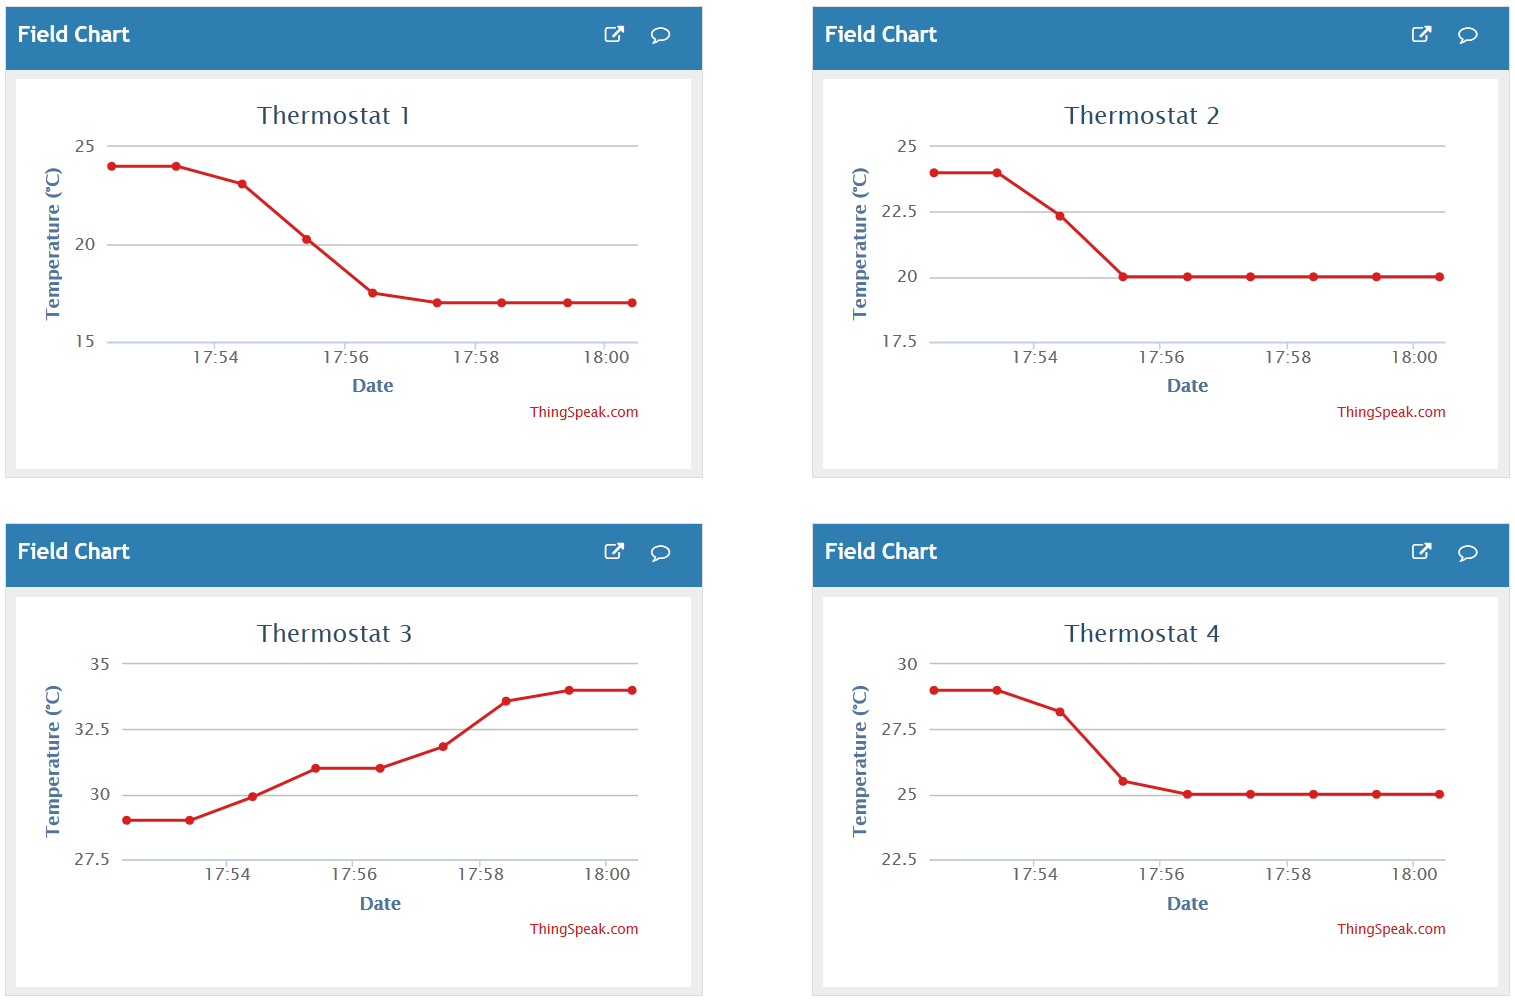
\includegraphics[width=0.8\linewidth]{images/thingspeak-thermostats.png}
\end{center}

\end{document}
